\documentclass{article}
\usepackage[margin=1.5cm,bottom=2cm]{geometry}
\usepackage{fancyhdr}
\usepackage{graphicx}
\usepackage[section]{placeins}
\pagestyle{fancy}
\usepackage{amsmath}

\begin{document}
\fancyhead[L]{ 
\includegraphics[width=2cm]{au_logo.png} }
\fancyhead[R]{PHYS 2240: General Physics II}
\fancyfoot[C]{\thepage}
\vspace*{0cm}
\begin{center}
	{\LARGE \textbf{Lab 5}}\\
	\vspace{.25cm}
	{\Large Sliding Friction}
	%\vspace{0.25cm}
	%{\Large Due: Friday, September 4}
\end{center}

\section*{Overview}
The goal of this lab is to calculate the coefficient of kinetic friction, $\mu_k$ for a block sliding on a surface.
\section*{Theory}
The resistive force of friction which opposes a moving object depends on the two materials in contact as well as the force with which one object presses on another, usually called the ``normal force'':
\begin{equation}
|\vec{F_f}|=\mu_k|\vec{F_N}|
\end{equation}
If I apply a force equal and opposite to $|\vec{F_f}|$, the system will move with constant velocity, as there will be no net force.
\section*{Predictions}
In this lab, you will investigate how the coefficient of kinetic friction $\mu_k$ depends on both (a) the mass of the sliding object and (b) the material of the sliding object. How do you expect $\mu_k$ to change with increasing mass? How do you expect $\mu_k$ to change when the material changes?
\section*{Setup}
At your lab station is a wooden block partially covered with felt, a long wooden track, and a force sensor. You will use this setup to experimentally measure the coefficient of friction for the wood track/wood block and for the wood track/felt block.

The basic idea is this: if you attach the force sensor to the block, and then pull such that the block moves at a constant velocity, then the force you measure with the sensor will be equal in magnitude to the frictional force. You will use this information to calculate $\mu_k$.

\begin{enumerate}
	\item First, wipe down the track with water and a paper towel (so that the surface will be as uniform as possible)
	\item Zero the force sensor and attach it to the block.
	\item Begin data collection and pull so that the block moves with constant velocity (as far as you can tell ``by eye'')
	\item Select the portion of your force vs time graph which most closely corresponds to the time when the block was moving with constant speed, and take the average. Record this value.
	\item Repeat steps 2-4 twice more, so that you have three estimates for the frictional force. The average of these three is your experimental value for frictional force.
	\item With your average frictional force estimate, use equation 1 to estimate $\mu_k$.
	\item Add some mass to your block, and repeat steps 2-5 to obtain another estimate for $\mu_k$
	\item Now, flip the block over (if you were using the felt side, switch to the wood side, and vice versa) and measure $\mu_k$ twice more, using the steps above.
\end{enumerate}
Figure \ref{fig1} shows a sample data table for the entire experiment (with completely made up numbers).
\begin{figure}
	\centering
	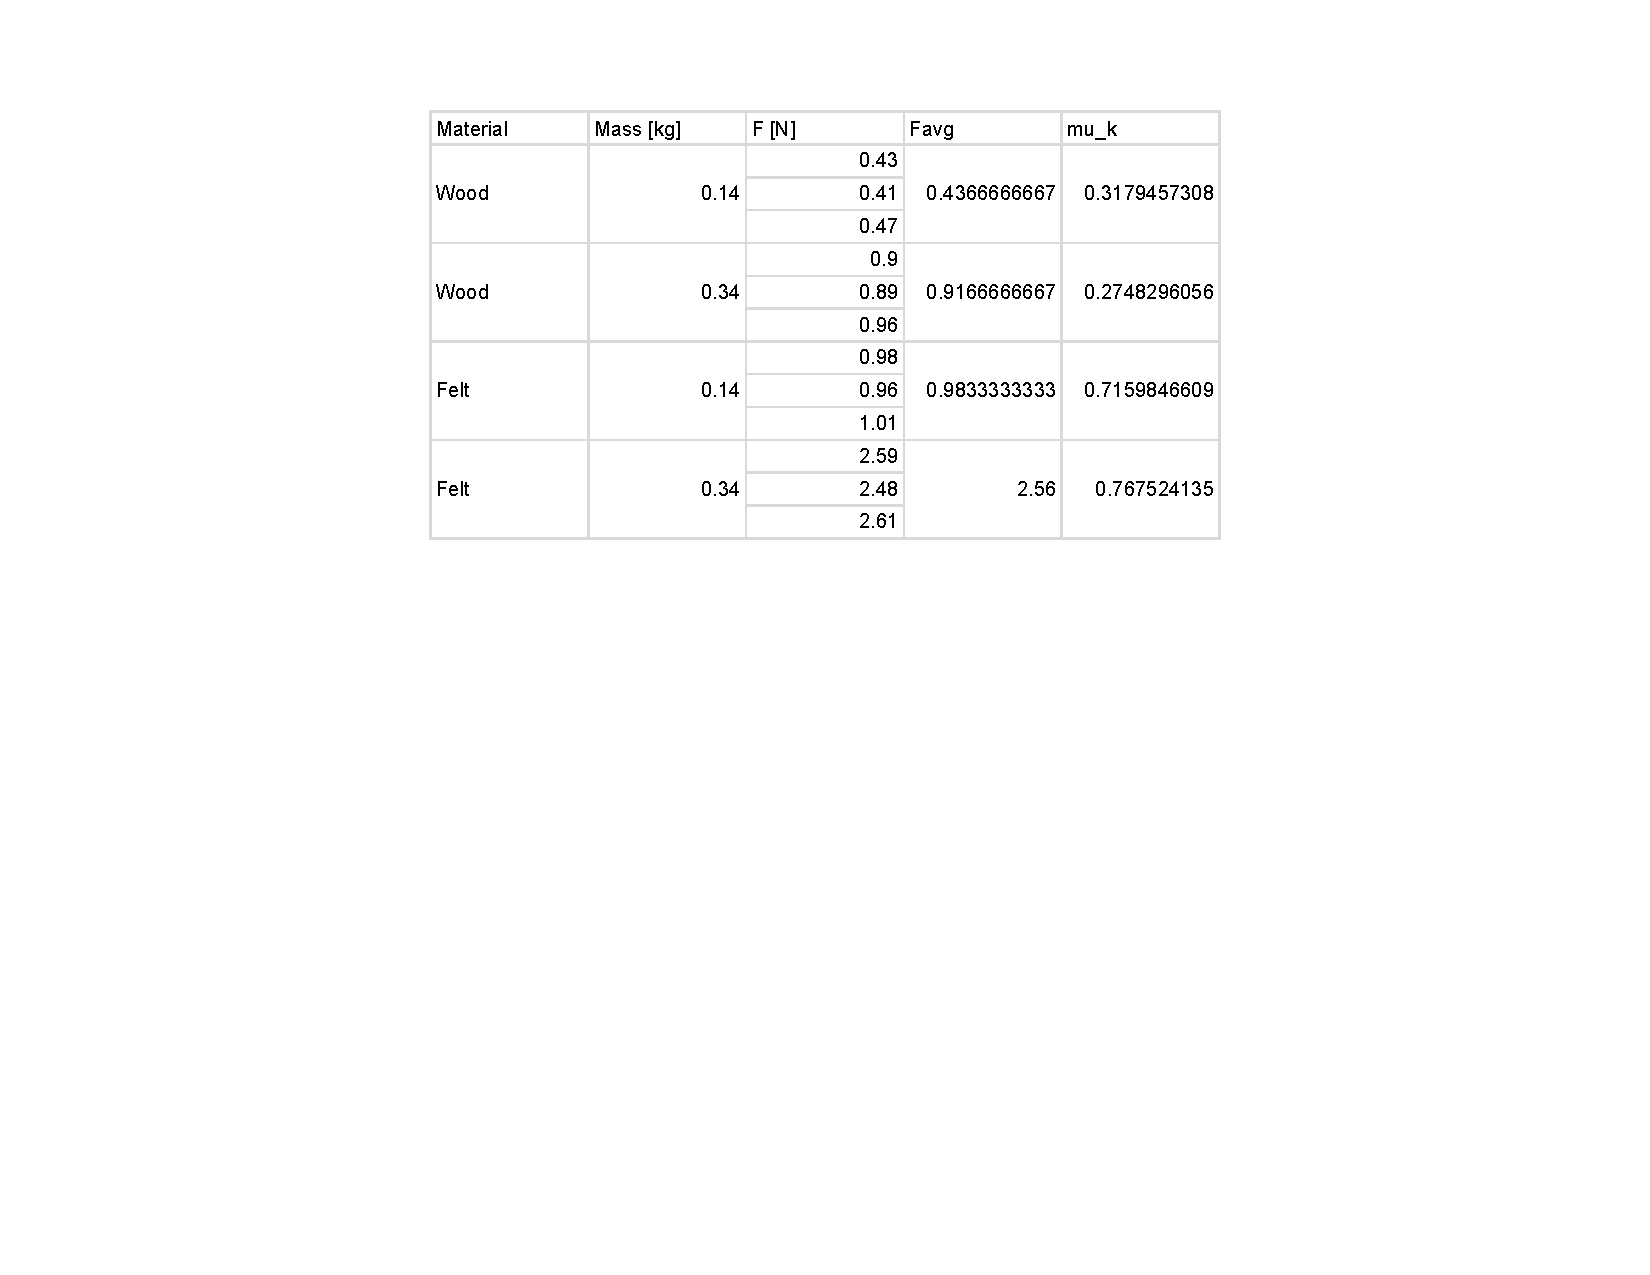
\includegraphics[width=10cm]{sample_table_friction}
	\label{fig1}
\end{figure}

\section*{Analysis}
\begin{itemize}
	\item How does the coefficient of friction depend on the mass of the sliding block? Is this what you expected? Explain.
	\item Did the coefficient of friction change between the wooden surface and the felt surface? Is this what you expected to happen? Explain.
	\item Would you expect $\mu_k$ to change if you placed the block on its narrow side (without changing the material)?
	\item What are a few possible sources of error or uncertainty that might affect the reliability of your results? Do not just say ``human error'', be more specific than that. List as many as you can.
\end{itemize}
\end{document}